\section*{Problema 14.34, Z}

\noindent Una masa $m$ está unida a un resorte de constante de fuerza de $75N/m$ y se deja oscilar. La figura muestra una gráfica de la velocidad $v_x$  como función del tiempo $t$. Determine $a)$ el periodo, $b)$ la frecuencia y $c)$ la frecuencia angular del movimiento. $d)$ ¿Cuál es la amplitud (en $cm$), y en qué momento la masa alcanza esta posición? $e)$ Determine la aceleración máxima de la amsa y los momentos en que se produce. $f)$ ¿Cuál es la masa $m$?

\begin{figure}[H]
	\centering
	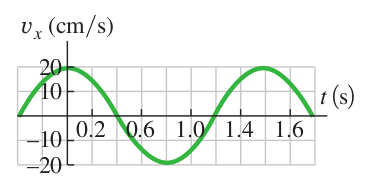
\includegraphics[scale=0.6]{./img/graph.png}
\end{figure}

%%%%